\section{Exemplos}

\subsection{Ambiente citação}

A partir da Nova Reforma do Ensino Industrial de 1959, as escolas industriais e técnicas foram transformadas em Escolas Técnicas Federais. Os cursos oferecidos tinham como objetivos

\begin{citacao}
	formar técnicos para o desempenho de funções de imediata assistência a engenheiros ou a administradores para o exercício de atividade em que as aplicações tecnológicas exigem do profissional dessa graduação \cite{Decreto47038BRASIL1959}.
\end{citacao}

\subsection{Referências explícitas}

É o caso em que você menciona explicitamente o autor da referência na sentença.

De acordo com \citeonline{Manfredi2002}, diversas abordagens retratam diferentes
concepções sobre a natureza do trabalho, dentre as quais se podem citar: a econômica, força
social de produção de bens e serviços; as categorias socioprofissionais, que originam as práticas
coletivas e determinam as relações entre os diferentes grupos, classes e setores da sociedade,
definindo parâmetros de identidade social e cultural; políticas governamentais, que têm por
base a regulação, o controle, a distribuição e a locação dos postos de trabalho.

\subsection{Referências implícitas}

São aquelas referências que não fazem parte do texto.

Diversas abordagens retratam diferentes
concepções sobre a natureza do trabalho, dentre as quais se podem citar: a econômica, força
social de produção de bens e serviços; as categorias socioprofissionais, que originam as práticas
coletivas e determinam as relações entre os diferentes grupos, classes e setores da sociedade,
definindo parâmetros de identidade social e cultural; políticas governamentais, que têm por
base a regulação, o controle, a distribuição e a locação dos postos de trabalho \cite{Manfredi2002}.

\subsection{Figuras}

Hoje, a Rede Federal conta com mais de 1 milhão de matrículas e 650 unidades de ensino, 38 Institutos Federais, 2 CEFETs, o Colégio Pedro II e 23 escolas técnicas distribuídas por centenas de municípios e por todas as unidades federativas. Toda essa estrutura suporta a oferta de mais de 11 mil cursos em todos os níveis de escolaridade, abrangendo desde a Educação Básica até o Doutorado. Do total de matrículas ofertadas pela rede, o ensino técnico representa 54,67\%, enquanto o ensino técnico integrado com o ensino médio alcança 21,69\% das matrículas \cite{PlataformaNiloPecanha2018}. A Figura \ref{fig:rede} mostra a espacialização da Rede Federal no ano de 2015.

\begin{figure}[h]
	\centering
	\caption{Espacialização da Rede Federal em 2015}
	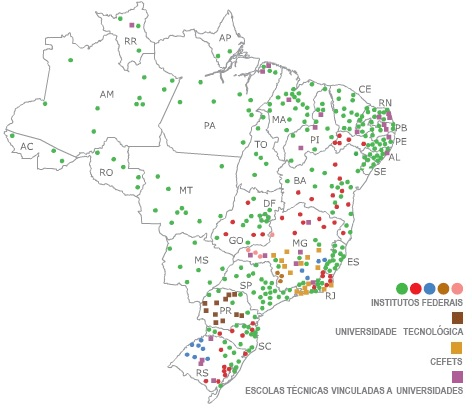
\includegraphics[width=0.8\textwidth, keepaspectratio]{rede.png}
	\legend{Adaptado de \citeonline{ifinstituicoes} pelo autor}
	\label{fig:rede}
\end{figure}

Seguindo as determinações da Lei nº 12.711 \cite{Lei12711}, as instituições da Rede Federal tem em sua política de seleção a reserva de 50\% das vagas a alunos oriundos integralmente do ensino médio público, sejam matriculados em cursos regulares ou da educação de jovens e adultos. Dessa reserva, metade delas estão destinadas para estudantes de escolas públicas com renda familiar bruta igual ou inferior a um salário mínimo e meio \textit{per capita}.

\subsection{Consulte o manual da classe \textsf{abntex2}}

Para exemplos adicionais de \abnTeX\ e \LaTeX, como inclusão de figuras,
fórmulas matemáticas, citações, e outros, consulte o documento
\citeonline{abntex2modelo}.

Consulte o manual da classe \textsf{abntex2} \cite{abntex2classe} para uma
referência completa das macros e ambientes disponíveis.